\documentclass[13pt]{article}
\usepackage[margin=1in]{geometry}
\usepackage{hyperref}
\usepackage{parskip}
\usepackage{amsmath}
\usepackage{graphicx}
\title{Image Compression Using SVD}
\author{EE25BTECH11005-ADITYA MISHRA}
\date{\today}

\begin{document}
\maketitle
\tableofcontents
\newpage
\section{Summary of Strang's Lecture}
\subsection{Overview}
The Singular Value Decomposition (SVD) breaks a real matrix \(A\) into
\[
A = U \Sigma V^{T}.
\]
\(U\) and \(V\) are orthogonal matrices. \(\Sigma\) is diagonal and contains non-negative singular values. SVD shows how a matrix can be rotated and scaled along main directions~\cite{strangSVD}.

\subsection{Main Idea}
SVD separates useful information from less important details. The larger singular values hold most of the data’s energy. Smaller ones often represent noise or fine details.  
The columns of \(V\) are eigenvectors of \(A^{T}A\), and the columns of \(U\) are eigenvectors of \(A A^{T}\). The squares of the singular values are the eigenvalues of these matrices.

\subsection{Use in Image Compression}
An image can be stored as a matrix of pixel values. Using SVD, we can keep only the top \(k\) singular values and the related vectors to get a low-rank version of the image. This reduces storage while keeping the main visual content.  
The Eckart–Young theorem~\cite{eckart1936approximation} states that this gives the best rank-\(k\) approximation in the Frobenius norm sense.

\section{Implemented Algorithm}
\subsection{Introduction}

I have implemented the \textbf{Lanczos Tridiagonalization with Implicit QR Iteration using Givens Rotations and Wilkinson Shift} algorithm. This method first reduces \(A^T A\) to a symmetric tridiagonal matrix through the Lanczos process and then applies the implicit QR algorithm to compute approximately the singular values of \(A\).
\subsection{Tridiagonalization and the Symmetric Lanczos Process}

The Lanczos process generates an orthonormal basis for the Krylov subspace
\[
\mathcal{K}_k(A, q_1) = \text{span}\{q_1, A q_1, A^2 q_1, \ldots, A^{k-1} q_1\},
\]
and a tridiagonal matrix \(T_k \in \mathbb{R}^{k \times k}\) such that
\[
A Q_k = Q_k T_k + \beta_{k+1} q_{k+1} e_k^T,
\]
where \(Q_k = [q_1, q_2, \ldots, q_k]\) has orthonormal columns and \(T_k = Q_k^T A Q_k\) is real symmetric and tridiagonal.


\subsection{Algorithm (Lanczos Tridiagonalization)}
Given a symmetric matrix \(A \in \mathbb{R}^{n \times n}\) and an initial unit vector \(q_1\):
\[
\begin{aligned}
&\beta_0 = 1, \quad q_0 = 0, \\
&\text{for } k = 1, 2, \ldots \\
&\quad \alpha_k = q_k^T A q_k, \\
&\quad r_k = (A - \alpha_k I) q_k - \beta_{k-1} q_{k-1}, \\
&\quad \beta_k = \|r_k\|_2, \\
&\quad q_{k+1} = r_k / \beta_k, \\
&\text{until } \beta_k = 0.
\end{aligned}
\]
The recurrence produces
\[
T_k =
\begin{bmatrix}
\alpha_1 & \beta_2 &        &        \\
\beta_2  & \alpha_2 & \ddots &        \\
         & \ddots & \ddots & \beta_k \\
         &        & \beta_k & \alpha_k
\end{bmatrix}.
\]
The vectors \(q_i\) are the \emph{Lanczos vectors}. If \(\beta_k = 0\), an invariant subspace of \(A\) has been found.

\subsection{Properties}
\begin{itemize}
\item The columns of \(Q_k\) span \(\mathcal{K}_k(A, q_1)\), and \(T_k = Q_k^T A Q_k\) gives a reduced symmetric eigenvalue problem.
\item The eigenvalues \(\theta_i\) of \(T_k\) are called \emph{Ritz values} and approximate the largest eigenvalues of \(A\).
\item If \(A\) is positive semidefinite, \(\sqrt{\theta_i}\) approximate the singular values of the original matrix.
\item Encountering a zero \(\beta_k\) indicates an exact invariant subspace; otherwise, the iteration continues until convergence.
\end{itemize}
\subsection{Pseudocode Summary}

\noindent
\textbf{Input:} \( A \in \mathbb{R}^{m \times n} \), target rank \( k \)  
\textbf{Output:} Approximate top-\(k\) singular values \( \sigma_1, \ldots, \sigma_k \)

\begin{verbatim}
# Lanczos tridiagonalization
v₁ = random_unit_vector(n)
β₁ = 0
for i = 1 to k
    w = Aᵀ * (A * vᵢ) - βᵢ * v_{i-1}
    αᵢ = vᵢᵀ * w
    w = w - αᵢ * vᵢ
    β_{i+1} = ||w||
    v_{i+1} = w / β_{i+1}
end
T = tridiagonal(α, β)

# Implicit QR iteration with Wilkinson shift
repeat until convergence:
    μ = wilkinson_shift(T)
    for j = 1 to k - 1
        (c, s) = givens(T[j,j] - μ, T[j+1,j])
        T = G_jᵀ * T * G_j
    end
    deflate if |T[k,k-1]| < ε
end
σ = sqrt(diag(T))
\end{verbatim}

\subsection{Summary}
The symmetric Lanczos algorithm reduces a large symmetric matrix to tridiagonal form using short recurrences and orthogonal vectors. The resulting \(T_k\) preserves the essential spectral information of \(A\) and forms the foundation for large-scale eigenvalue and SVD computations.
\section{Algorithm Comparison}

\begin{table}[h!]
\centering
\renewcommand{\arraystretch}{1.3}
\setlength{\tabcolsep}{5pt}
\begin{tabular}{|p{3.5cm}|p{3cm}|p{3cm}|p{2.2cm}|p{5.2cm}|}
\hline
\textbf{Algorithm} &
\textbf{Reduction Type} &
\textbf{Stability Mechanism} &
\textbf{Complexity} &
\textbf{Remarks} \\
\hline
\textbf{Lanczos Tridiagonalization + Implicit QR (Givens + Wilkinson Shift)} &
Tridiagonal reduction of \(A^T A\) &
Givens rotations with reorthogonalization &
\(O(k n^2)\) &
Fast, stable, and shift–accelerated; preserves sparsity; suitable for large SVD and image compression. \\
\hline
\textbf{Golub--Kahan Bidiagonalization} &
Two–sided bidiagonal reduction of \(A\) &
Orthogonal recurrences for \(A\) and \(A^T\) &
\(O(k n^2)\) &
Two–sided extension of Lanczos; forms basis of LSQR and truncated SVD solvers; stable for rectangular or sparse matrices. \\
\hline
\textbf{Lanczos with Bidiagonalization} &
Bidiagonal reduction via Krylov subspace &
Three–term orthogonal recurrence &
\(O(k n^2)\) &
Efficient for large sparse \(A\); used in partial SVD; sensitive to loss of orthogonality. \\
\hline
\textbf{QR with Householder Reduction} &
Full Hessenberg / bidiagonal reduction &
Householder reflectors &
\(O(n^3)\) &
Highly stable for dense problems; destroys sparsity; standard in LAPACK routines. \\
\hline
\textbf{Standard QR Algorithm} &
Hessenberg or tridiagonal form &
Orthogonal similarity transforms &
\(O(n^3)\) &
General solver for dense matrices; slower without shift strategy. \\
\hline
\textbf{Standard QL Algorithm} &
Tridiagonal form &
Orthogonal transformations &
\(O(n^3)\) &
Processes eigenvalues in reverse order; similar cost to QR. \\
\hline
\textbf{Jacobi Method} &
Successive plane rotations to diagonal form &
Orthogonal rotations &
\(O(n^3)\) &
High accuracy but computationally heavy; impractical for large sparse systems. \\
\hline
\textbf{Bisection (Eigenvalues only)} &
Requires tridiagonal input &
Sturm sequence count &
\(O(n^2 \log n)\) &
Stable and robust; computes eigenvalues only, not eigenvectors. \\
\hline
\textbf{Power Iteration} &
None (direct iteration) &
Normalization per step &
\(O(n^2 k)\) &
Low cost but converges to a single dominant eigenvalue; poor for clustered spectra. \\
\hline
\textbf{Hardcoded Direct Method} &
Explicit analytical computation &
Exact arithmetic only &
\(O(1)\) for fixed \(n\) &
Non-scalable and inflexible; valid only for small static matrices. \\
\hline
\end{tabular}
\caption{Comparison between different Algorithms}
\label{tablealgo}
\end{table}

The above table compares the implemented \textbf{Lanczos Tridiagonalization with Implicit QR (Givens + Wilkinson Shift)} algorithm against several classical eigenvalue and SVD methods in terms of computational features and practical performance.
\subsection{Justification for choosing Lanczos Tridiagonalization amongst others}

Of these Algorithms , prioritizing accuracy and  time complexity before implementation difficulty, the one I found most suitable was \textbf{Golub-Kahan Bidiagonalization} but due to its increased implementation difficulty as compared to others that were similar in performance and the lack of sufficient time to fully implement it, I had to move to the next two suitable algorithms that were \textbf{Lanczos Tridiagonalization} and \textbf{Lanczos Bidiagonalization}. Since \textbf{Lanczos Bidiagonalization} was sensitive to loss of orthogonality and rest all aspects of comparison such as implementation difficulty, computational complexity, implementation difficulty were almost similar, I chose \textbf{Lanczos Tridiagonalization + QR using Givens Rotation and Wilkinson Shift}.
\section{Reconstructed images for different k}
\begin{figure}[h]
\centering
\begin{tabular}{ccc}

\includegraphics[width=0.3\textwidth]{figs/globe.jpg} & 
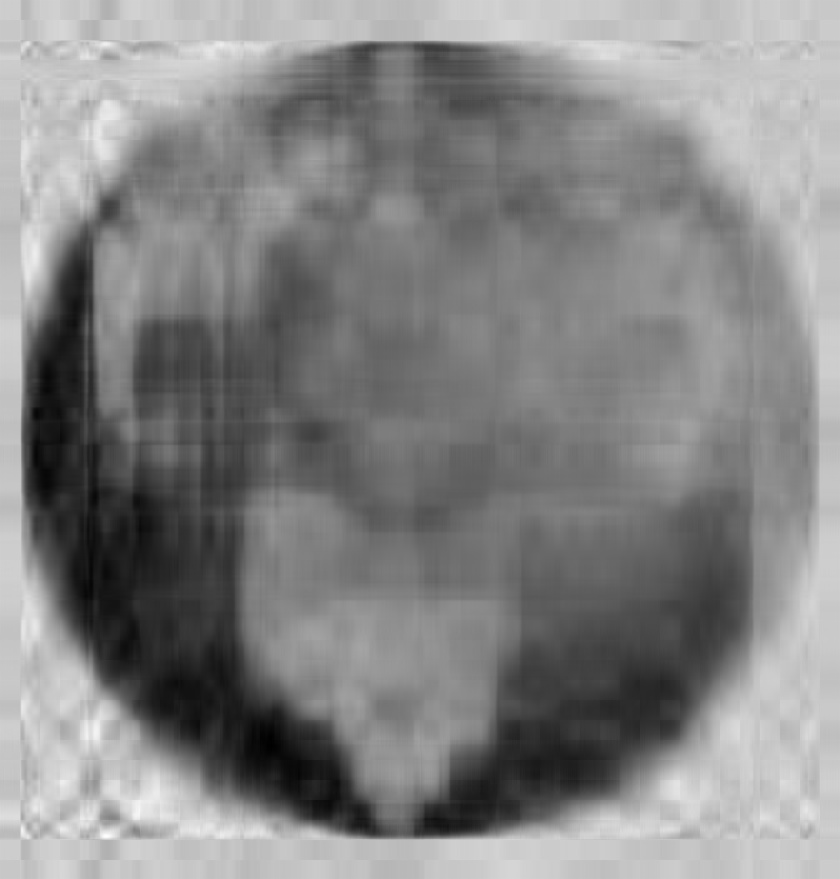
\includegraphics[width=0.3\textwidth]{figs/globek10.jpg} &

\includegraphics[width=0.3\textwidth]{figs/globek20.jpg} \\
Original & $k = 10$ & $k = 20$ \\[1em]

\includegraphics[width=0.3\textwidth]{figs/globek50.jpg} &

\includegraphics[width=0.3\textwidth]{figs/globek100.jpg} &
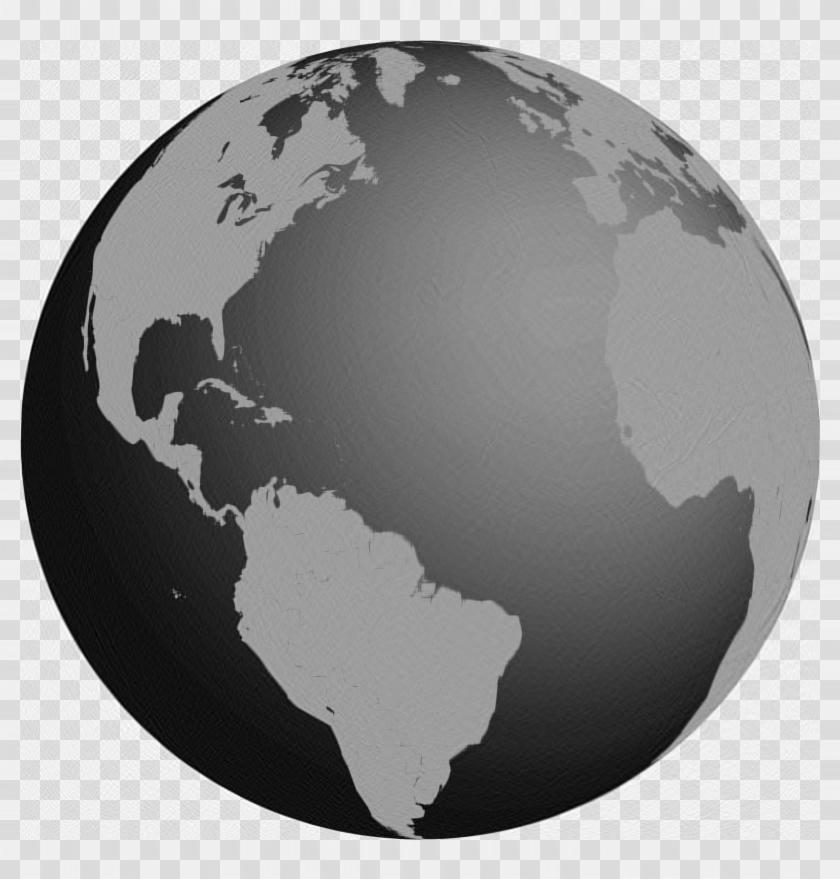
\includegraphics[width=0.3\textwidth]{figs/globek200.jpg} \\
$k = 50$ & $k = 100$ & $k = 200$  \\
\end{tabular}
\caption{SVD Image Compression Results for globe.jpg Various Values of $k$}
\label{fig:svd_compression_globe}
\end{figure}
\newpage
\begin{figure}[h]
\centering
\begin{tabular}{ccc}
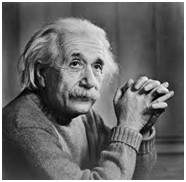
\includegraphics[width=0.3\textwidth]{figs/einstein.jpg} &
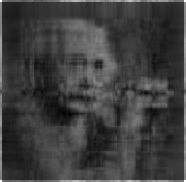
\includegraphics[width=0.3\textwidth]{figs/einsteink10.jpg} &
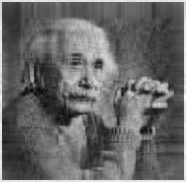
\includegraphics[width=0.3\textwidth]{figs/einsteink20.jpg} \\
Original & $k = 10$ & $k = 20$ \\[1em]
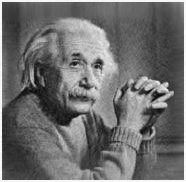
\includegraphics[width=0.3\textwidth]{figs/einsteink50.jpg} &
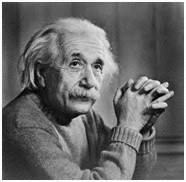
\includegraphics[width=0.3\textwidth]{figs/einsteink100.jpg} &
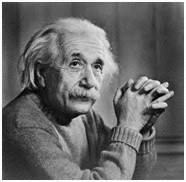
\includegraphics[width=0.3\textwidth]{figs/einsteink100.jpg} \\
$k = 50$ & $k = 100$ &  \\ % no k=200 available
\end{tabular}
\caption{SVD Image Compression Results for einstein.jpg with Various Values of $k$}
\label{fig:svd_compression_einstein}
\end{figure}
\newpage
\begin{figure}[h]
\centering
\begin{tabular}{ccc}
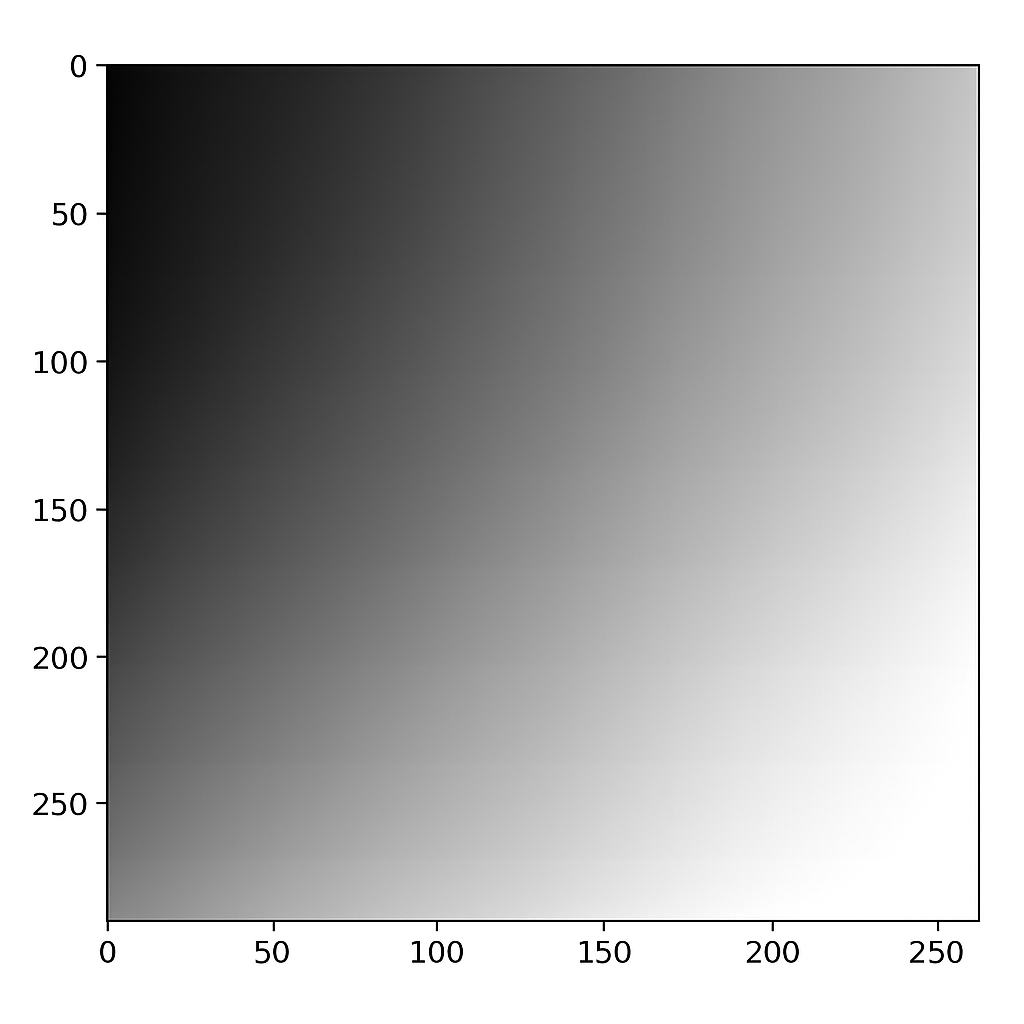
\includegraphics[width=0.3\textwidth]{figs/greyscale.png} &
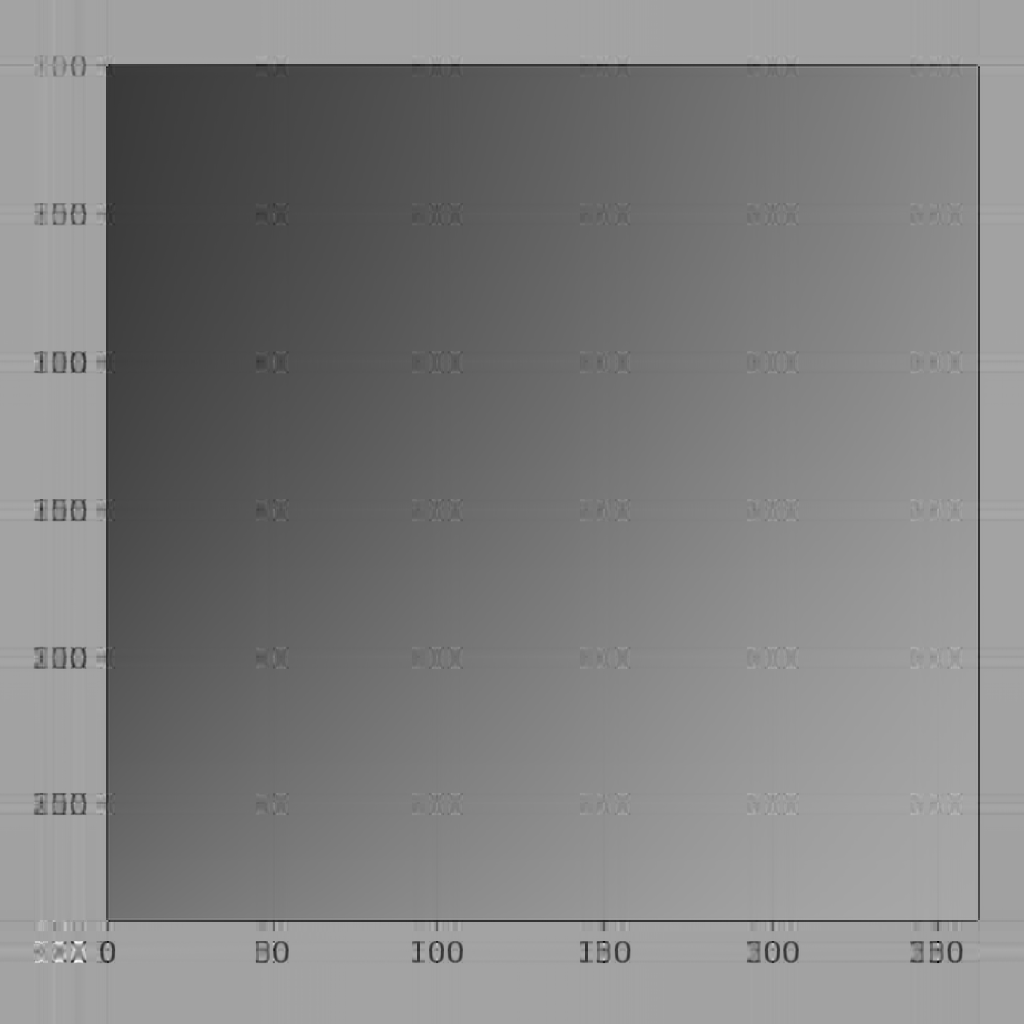
\includegraphics[width=0.3\textwidth]{figs/greyscalek10.png} &
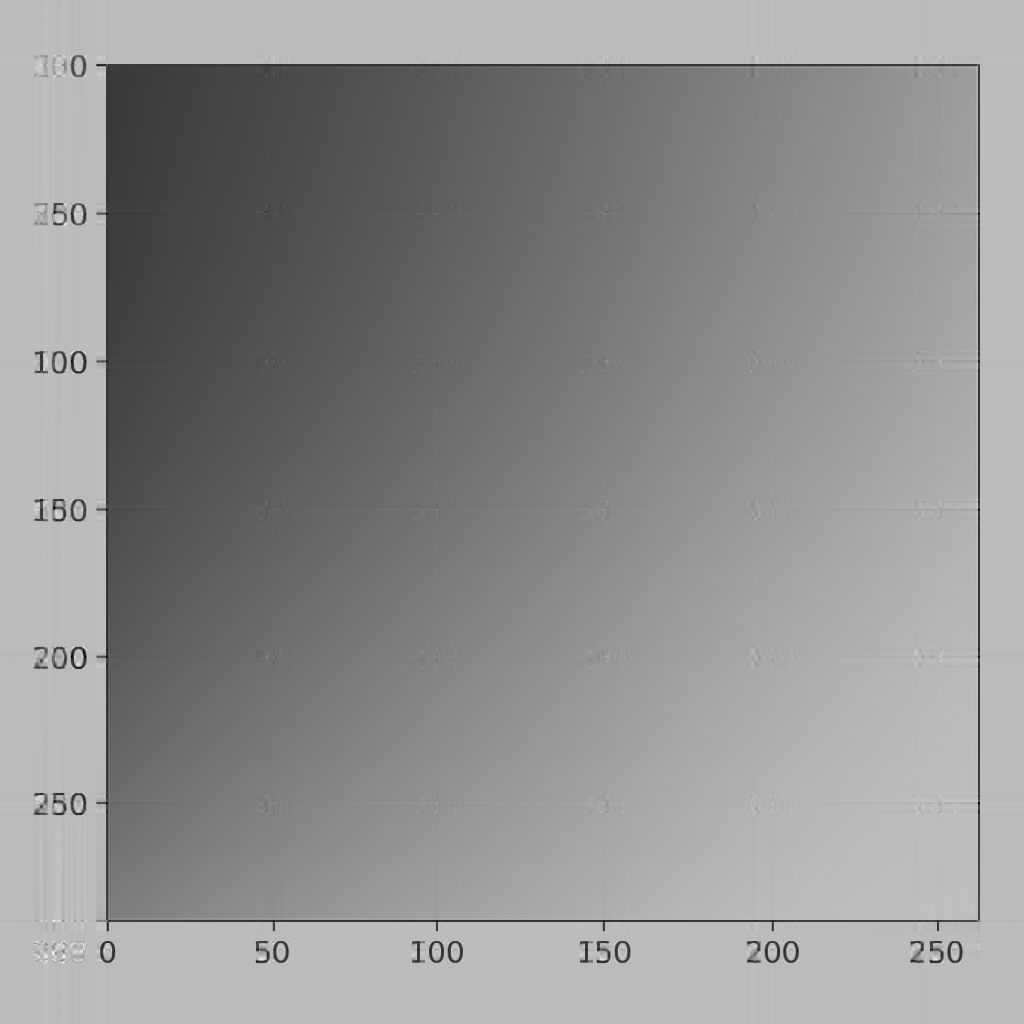
\includegraphics[width=0.3\textwidth]{figs/greyscalek20.png} \\
Original & $k = 10$ & $k = 20$ \\[1em]
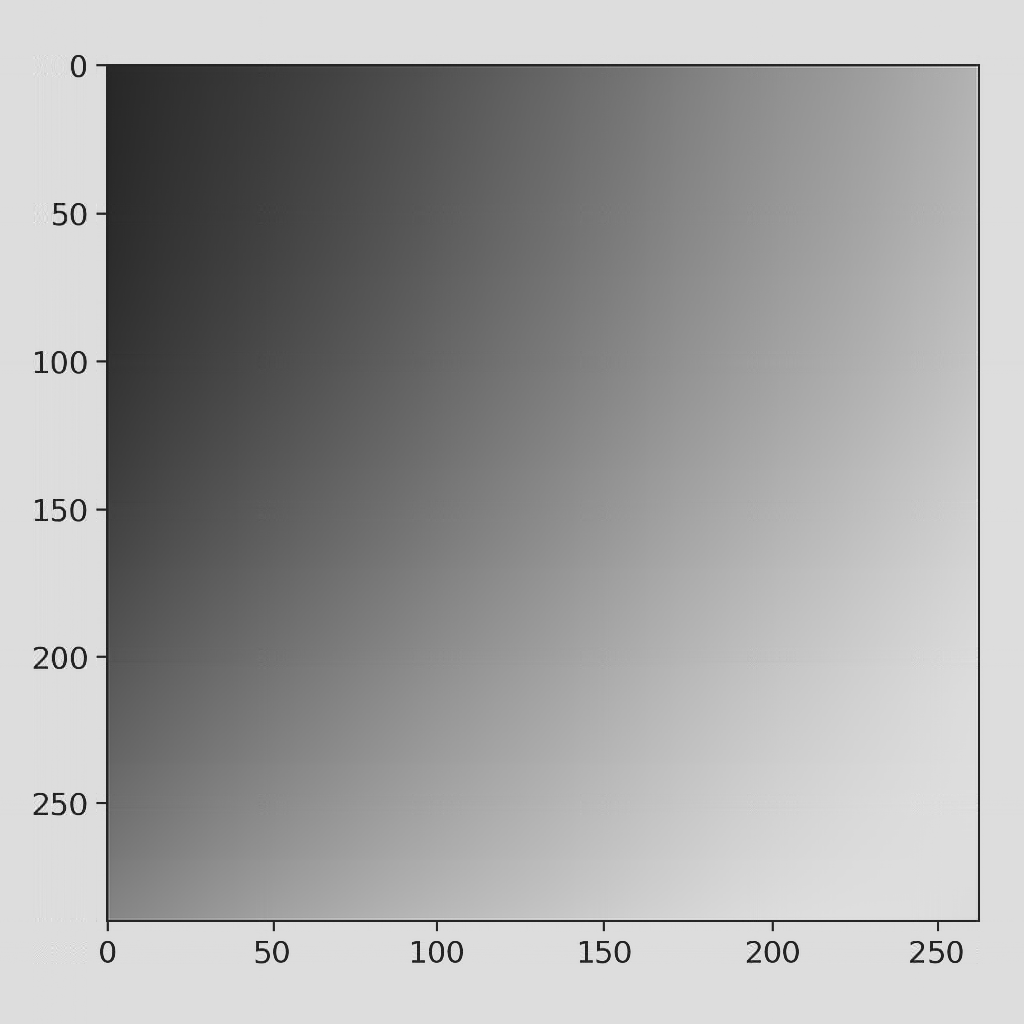
\includegraphics[width=0.3\textwidth]{figs/greyscalek50.png} &
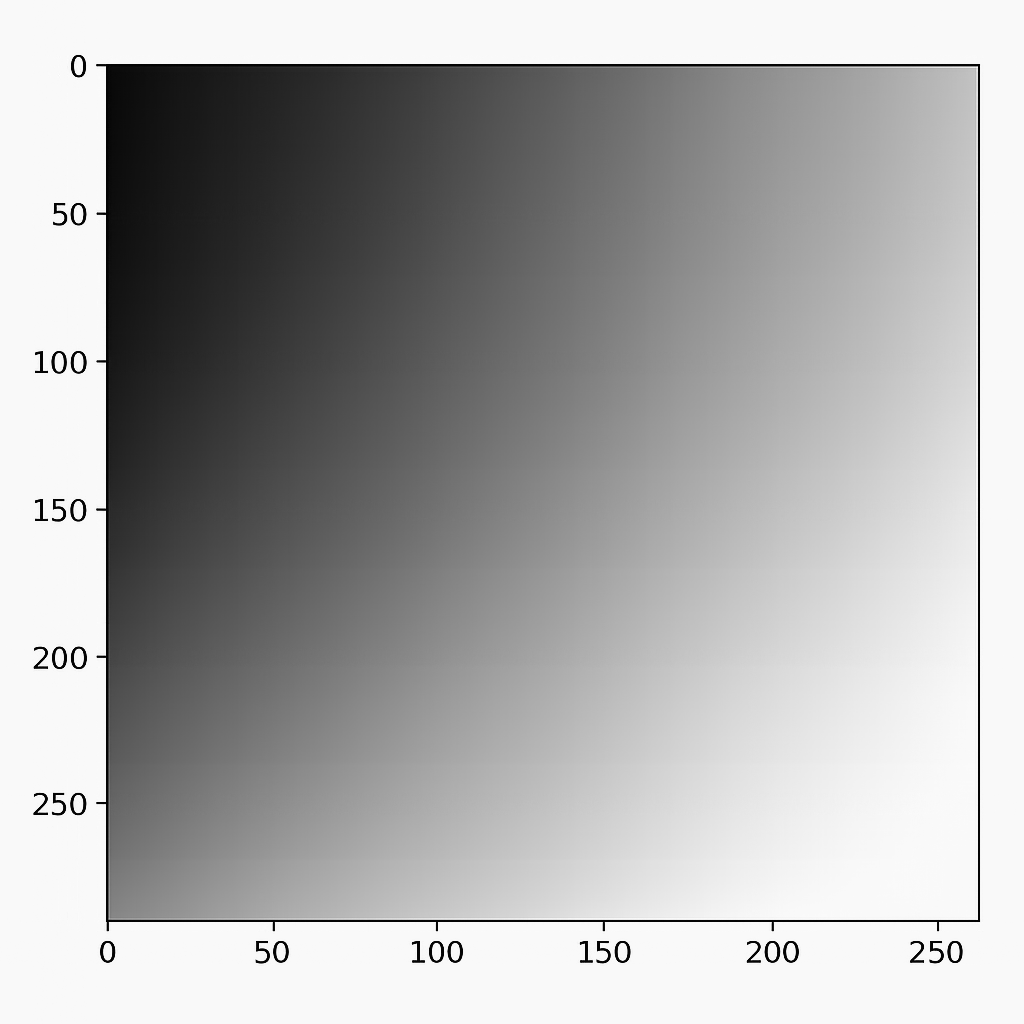
\includegraphics[width=0.3\textwidth]{figs/greyscalek100.png} &
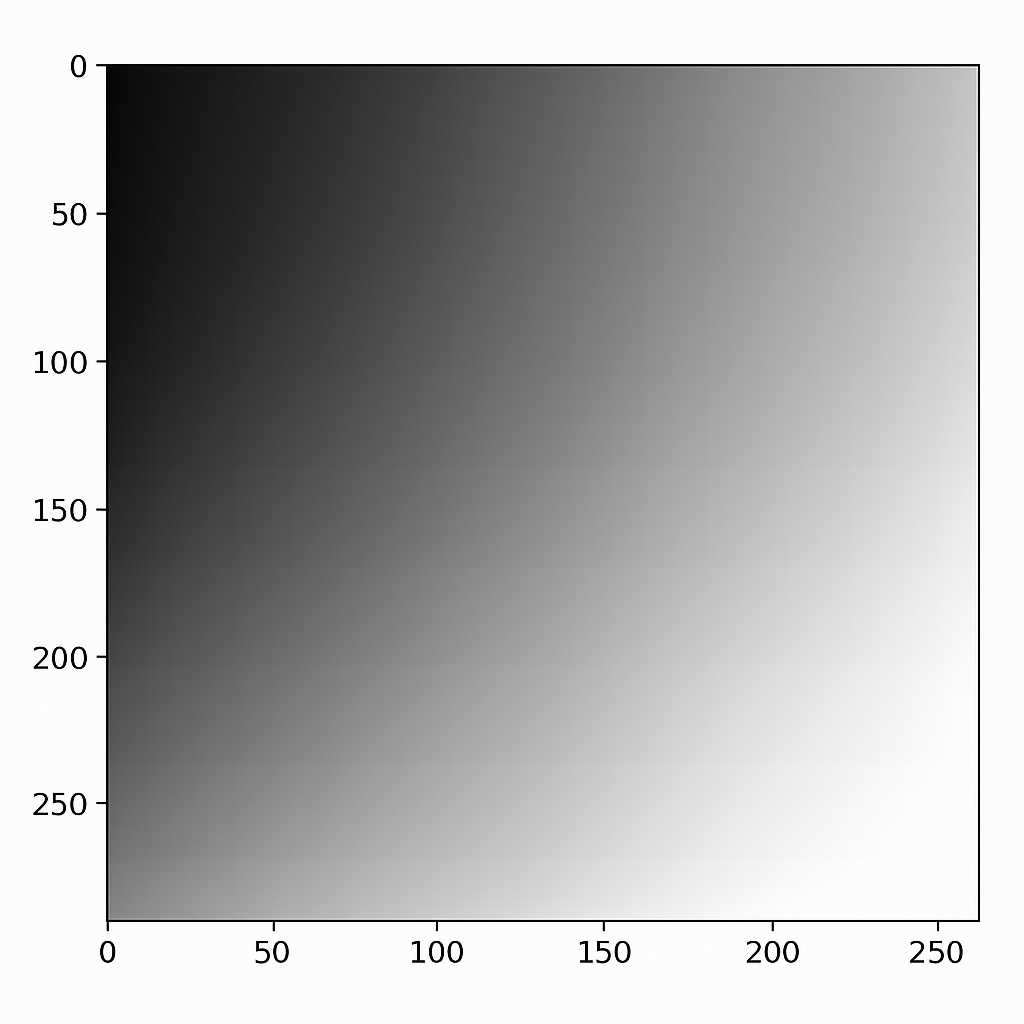
\includegraphics[width=0.3\textwidth]{figs/greyscalek200.png} \\
$k = 50$ & $k = 100$ & $k = 200$ \\
\end{tabular}
\caption{SVD Image Compression Results for \texttt{greyscale.png} with Various Values of $k$}
\label{fig:svd_compression_greyscale}
\end{figure}

\section{Error}
The Frobenius norm error $\|A - A_k\|_F$ quantifies the difference between the original image matrix $A$ and its rank-$k$ approximation $A_k$ obtained from the truncated SVD. 
It is computed as the square root of the sum of squared pixel-wise differences between $A$ and $A_k$. 
A smaller value of $\|A - A_k\|_F$ indicates a closer approximation and better preservation of image details. 
As $k$ increases, more singular values are retained, reducing the error and improving the reconstruction quality.

\include{tables/errors}

\section{Trade-off between k, image quality, and compression}
There is a tradeoff between the value of $k$, image quality and compression ratio since increasing $k$ retains more singular values and improves image quality but reduces compression efficiency while decreasing $k$ increases compression but causes more loss of detail and blurring in the reconstructed image
\section{Bibliography}
\begin{thebibliography}{9}

\bibitem{strangSVD}
G.~Strang, ``Singular Value Decomposition,'' \textit{MIT OpenCourseWare Lecture},\\
\url{https://youtu.be/TX_vooSnhm8}

\bibitem{eckart1936approximation}
C.~Eckart and G.~Young, ``The Approximation of One Matrix by Another of Lower Rank,'' 
\textit{Psychometrika}, vol.~1, no.~3, pp.~211--218, 1936.\\
Available at: \url{https://doi.org/10.1007/BF02288367}

\bibitem{golubvanloan}
G.~H.~Golub and C.~F.~Van~Loan, \textit{Matrix Computations}, 4th~ed.,\\
Johns Hopkins University Press, Baltimore, 2012.\\
Referenced sections: §§5.2.5, 8.6, and 10.4.

\end{thebibliography}


\end{document}
